\documentclass[11pt,a4paper]{article}
\usepackage[margin=18mm]{geometry}
\usepackage{amsmath,amssymb,mathtools}
\usepackage{booktabs,array,enumitem}
\usepackage[dvipsnames]{xcolor}
\usepackage{graphicx,listings,tikz,float,needspace}
\usetikzlibrary{arrows.meta,positioning}
\usepackage[most]{tcolorbox}
\usepackage{hyperref}
\hypersetup{colorlinks=true,urlcolor=MidnightBlue,linkcolor=MidnightBlue}
\setlength{\parindent}{0pt}\setlength{\parskip}{4pt}
\newcommand{\course}{PHY4605 Computational Methods in Physics}
\newcommand{\units}[1]{\,\mathrm{#1}}
\newtcolorbox{keybox}{colback=RoyalBlue!5,colframe=RoyalBlue!65!black,boxrule=.7pt,arc=2mm}
\newtcolorbox{checkbox}{colback=ForestGreen!5,colframe=ForestGreen!55!black,boxrule=.7pt,arc=2mm}
\newtcolorbox{aibox}{colback=BurntOrange!7,colframe=BurntOrange!80!black,boxrule=.7pt,arc=2mm}
\lstdefinestyle{matlabstyle}{language=Matlab,basicstyle=\ttfamily\footnotesize,keywordstyle=\color{RoyalBlue!75!black},commentstyle=\color{ForestGreen!55!black},stringstyle=\color{BurntOrange!80!black},numbers=left,numberstyle=\scriptsize\color{black!50},numbersep=5pt,frame=single,rulecolor=\color{RoyalBlue!25},backgroundcolor=\color{RoyalBlue!3},showstringspaces=false,columns=fullflexible,keepspaces=true,breaklines=true}
\begin{document}
{\large\textsc{\course}}\\[-2pt]
{\small Learning Note \textbar\ Week 7}\par\vspace{4pt}
{\LARGE\bfseries Numerical Integration}\par\vspace{3pt}
\textit{Estimate a physically accumulated quantity from sampled values, then test whether refinement and an independent reference support the result.}

\begin{keybox}\textbf{Physical question.} A force changes continuously with time and gradually decays. How can sampled force values estimate the total impulse delivered from $t=0$ to $t=2.0\units{s}$?\end{keybox}

\section*{Core learning outcomes}
\begin{enumerate}[nosep,leftmargin=5mm]
\item connect area under a physical curve to an accumulated quantity, limits, and units;
\item trace a trapezoidal estimate and the equivalent MATLAB \texttt{trapz(x,y)} calculation; and
\item validate a numerical integral using refinement, an analytic/reference value, and simple error.
\end{enumerate}

\section*{1. Integration means physical accumulation}
In calculus, an integral is often introduced as area under a curve. In computational physics, that area usually represents a physical quantity. For a force that varies with time,
\[
J=\int_{t_a}^{t_b}F(t)\,dt
\]
is the \textbf{impulse} delivered over the stated interval.

The axes carry the unit of the integral. Force is measured in newtons and time in seconds, so
\[
\units{N}\times\units{s}=\units{N\,s},
\]
which is also equivalent to the momentum unit $\units{kg\,m\,s^{-1}}$. The limits $t_a$ and $t_b$ are part of the physical question: changing them changes what has been accumulated.

\begin{checkbox}\textbf{Prediction checkpoint.} If the force remains positive from $0$ to $2.0\units{s}$, the impulse must be positive. If the force starts at $12\units{N}$ and then decays, the impulse must also be smaller than the rectangle $12\units{N}\times2\units{s}=24\units{N\,s}$.\end{checkbox}

\section*{2. Reuse a simple decaying-force model}
Use
\[
F(t)=F_0e^{-t/\tau},
\]
with
\[
F_0=12\units{N},\qquad \tau=0.8\units{s},\qquad 0\le t\le2.0\units{s}.
\]
The force is largest at the start and decreases smoothly while remaining positive. We want the accumulated impulse
\[
J=\int_0^{2.0}F(t)\,dt.
\]

For validation later, this teaching model has an analytic integral:
\[
J_{\mathrm{exact}}=F_0\tau\left(1-e^{-T/\tau}\right)
=8.8119840132\units{N\,s}.
\]
This value is the independent reference, not the numerical method.

\section*{3. A numerical integral only sees samples}
A computer does not need the entire continuous curve to apply a basic quadrature rule. It uses values at selected coordinates. With four equal intervals between $0$ and $2.0\units{s}$,
\[
\Delta t=\frac{2.0-0}{4}=0.5\units{s},
\]
so the five sample coordinates are $0$, $0.5$, $1.0$, $1.5$, and $2.0\units{s}$.

\begin{center}\small
\begin{tabular}{rr}
\toprule
$t$ (s) & $F(t)$ (N)\\
\midrule
0.0 & 12.0000\\
0.5 & 6.4231\\
1.0 & 3.4381\\
1.5 & 1.8403\\
2.0 & 0.9850\\
\bottomrule
\end{tabular}
\end{center}

\begin{figure}[H]
\centering
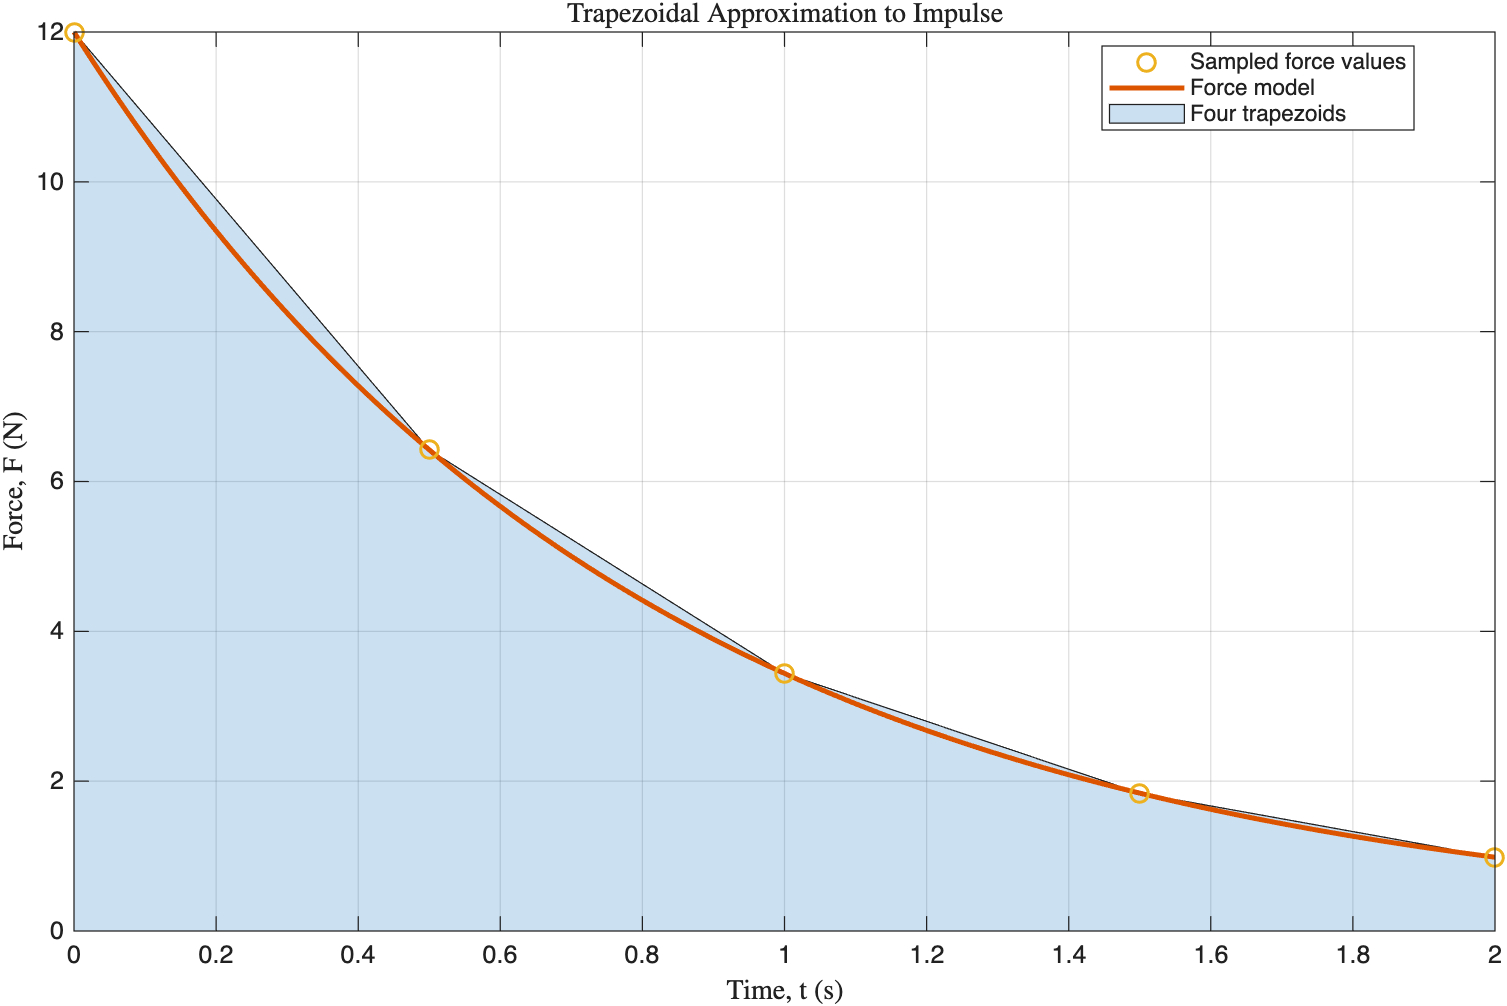
\includegraphics[width=.60\linewidth]{../matlab/assets/week07_impulse_trapezoids.png}
\caption{Week 7 force-time model: five samples define four trapezoids whose total area estimates the impulse.}
\end{figure}

\section*{4. One trapezoid is width times average height}
Between two neighbouring samples, approximate the curved force by a straight segment. For samples $F_i$ and $F_{i+1}$ separated by $\Delta t$,
\[
A_i\approx \Delta t\,\frac{F_i+F_{i+1}}{2}.
\]
For the first interval, from $0$ to $0.5\units{s}$,
\[
A_1\approx0.5\,\frac{12.0000+6.4231}{2}
\approx4.6058\units{N\,s}.
\]
The unit is already the unit of impulse because the trapezoid width is in seconds and its height is in newtons.

\section*{5. Add the trapezoids for a composite estimate}
For uniform spacing, the four trapezoids can be collected into the composite form
\[
J_{\mathrm{trap}}
=\Delta t\left[
\frac{1}{2}F_0+F_1+F_2+F_3+\frac{1}{2}F_4
\right].
\]
Using the five sampled values above,
\[
J_{\mathrm{trap}}\approx9.0969821492\units{N\,s}.
\]
This result is positive and below $24\units{N\,s}$, so it passes the basic sign and bound checks. Those checks are useful, but they do not yet tell us whether the approximation is accurate enough.

\section*{6. Pseudocode before MATLAB}
\begin{enumerate}[nosep,leftmargin=7mm]
\item state the accumulated quantity, integration limits, and expected unit;
\item choose a supplied number of intervals;
\item create sample coordinates between the fixed limits;
\item evaluate the force at those coordinates;
\item add trapezoid areas between neighbouring samples;
\item repeat at finer supplied resolutions without changing the force model;
\item compare the estimates with an independent reference; and
\item report the final integral with its unit, error, and physical meaning.
\end{enumerate}

\Needspace{18\baselineskip}
\section*{7. MATLAB \texttt{trapz} performs the same accumulation}
The coarse calculation can be written explicitly and then checked against MATLAB's built-in trapezoidal integration function:
\begin{lstlisting}[style=matlabstyle]
F0_N = 12;
tau_s = 0.8;
T_s = 2.0;
n = 4;
t_s = linspace(0,T_s,n+1);
F_N = F0_N*exp(-t_s/tau_s);
dt_s = T_s/n;
J_manual_Ns = dt_s*(0.5*F_N(1) + ...
    sum(F_N(2:end-1)) + 0.5*F_N(end));
J_trapz_Ns = trapz(t_s,F_N);
\end{lstlisting}

The call \texttt{trapz(t\_s,F\_N)} matters: the first argument supplies the physical coordinates and therefore the actual spacing between samples. The manual and \texttt{trapz} estimates should agree for the same data.

\begin{aibox}\textbf{Runnable does not mean physically correct.} The call \texttt{trapz(F\_N)} runs, but MATLAB then assumes unit spacing between samples. If the real sample spacing is $0.5\units{s}$, reporting that raw result directly as an impulse silently loses the physical time scale.\end{aibox}

\section*{8. Refine the sampling without changing the physics}
Now keep $F_0$, $\tau$, and the integration limits fixed while increasing only the number of intervals. This isolates the effect of numerical resolution.

\begin{center}\small
\begin{tabular}{rrrrr}
\toprule
Intervals & $\Delta t$ (s) & $J_{\mathrm{trap}}$ (N s) & abs. error (N s) & rel. error (\%)\\
\midrule
4  & 0.500 & 9.0969821 & 0.2849981 & 3.2342\\
8  & 0.250 & 8.8835797 & 0.0715957 & 0.8125\\
16 & 0.125 & 8.8299047 & 0.0179207 & 0.2034\\
\bottomrule
\end{tabular}
\end{center}

The estimates move toward the same analytic reference as the sample spacing is reduced. For this smooth model and these supplied resolutions, the error also decreases each time the spacing is halved.

\section*{9. Core validation: refinement plus reference comparison}
The finest supplied estimate is
\[
J_{16}=8.8299047499\units{N\,s}.
\]
Compared with the analytic reference,
\[
\left|J_{16}-J_{\mathrm{exact}}\right|
=0.0179207367\units{N\,s},
\]
and the relative error is approximately
\[
0.203\%.
\]

\begin{checkbox}\textbf{Validation statement.} The numerical impulse remains positive and below the physical upper bound, and the trapezoidal estimate approaches the analytic result as the sampling is refined. At 16 intervals the result differs from the analytic reference by about $0.203\%$, supporting the estimate for the stated model and limits.\end{checkbox}

\section*{10. Interpret the number physically}
An impulse of about $8.83\units{N\,s}$ corresponds to a momentum change of about $8.83\units{kg\,m\,s^{-1}}$ in the positive force direction over $0$ to $2.0\units{s}$. This interpretation is conditional on the stated force model and limits; numerical precision cannot repair an inappropriate model.

\section*{Working exposure: Simpson comparison and convergence evidence}
A supplied eight-interval Simpson result, $J_{\mathrm{Simpson}}=8.8124455163\units{N\,s}$, is close to the same exact reference. Treat it only as comparison evidence: Core work does not require deriving or independently implementing Simpson's rule. In the trapezoidal table, halving $\Delta t$ reduces error by about a factor of four; describe that observed pattern without deriving its formal order.

\section*{Optional stretch}
Optional extensions are quadrature error-order derivation, independent composite-rule comparison, and adaptive quadrature; none is required for the Core pathway.

\section*{Three takeaways}
\begin{enumerate}[nosep,leftmargin=6mm]
\item A numerical integral represents physical accumulation over explicit limits, and its unit combines the two axis units.
\item The trapezoidal rule sums areas between neighbouring samples; \texttt{trapz(x,y)} uses their supplied coordinates.
\item Refine the sampling and compare with a reference before trusting the accumulated result.
\end{enumerate}

\begin{keybox}\textbf{Preparation for the practical.} Transfer the same reasoning to impulse, work, and charge. For each context, identify the accumulated quantity, limits, axis units, trapezoidal sampling/refinement plan, and validation reference.\end{keybox}
\end{document}
